\documentclass[12pt,a4paper]{article}

% Packages
\usepackage[utf8]{inputenc}
\usepackage[T1]{fontenc}
\usepackage{lmodern}
\usepackage[margin=2.5cm]{geometry}
\usepackage{graphicx}
\usepackage{booktabs}
\usepackage{hyperref}
\usepackage{amsmath}
\usepackage{amsfonts}
\usepackage{amssymb}
\usepackage{caption}
\usepackage{subcaption}
\usepackage{xcolor}
\usepackage{listings}
% Hyperref setup
\hypersetup{
    colorlinks=true,
    linkcolor=blue,
    filecolor=magenta,
    urlcolor=cyan,
    citecolor=blue,
}

\begin{document}

% Title Page
\begin{titlepage}
    \centering
    \vspace*{2cm}
    {\Large\bfseries Multimedia Information Processing, Spring 2026\par}
    \vspace{1.5cm}
    {\Huge\bfseries Course Project Midterm Progress Report\par}
    \vspace{2cm}
    {\LARGE\bfseries Project Title: MoodWave -- Real-Time Music Emotion Recognition with Audio-Reactive Visualization\par}
    \vspace{1.5cm}
    {\large
    \textbf{Group Number:} [Your Group ID]\\[0.5em]
    \textbf{Team Members:} [Member A (Leader), Member B, Member C]\\[0.5em]
    \textbf{Supervisor:} [Advisor's Name]\\[0.5em]
    \textbf{Submission Date:} April 17, 2026\par}
    \vfill
\end{titlepage}

\tableofcontents
\newpage

% ============================================================
\section{Project Overview}
% ============================================================

Music is a universal language that evokes powerful emotional responses in listeners. However, quantifying and translating these emotional qualities into real-time interactive visual experiences remains a challenging problem at the intersection of audio signal processing, machine learning, and multimedia art. The goal of the \textbf{MoodWave} project is to build an end-to-end system that analyzes the emotional content of music in real time and drives an audio-reactive visualization in TouchDesigner (TD), a node-based visual programming environment widely used for interactive multimedia installations. \\

The theoretical foundation of this project is rooted in the well-established psychological framework that represents emotional states along two orthogonal dimensions (Russell, 1980): \textbf{valence} (pleasantness, ranging from negative to positive) and \textbf{arousal} (intensity, ranging from calm to excited). By predicting continuous valence and arousal values from raw audio waveforms, we can map any musical excerpt onto a two-dimensional emotion space. This mapping subsequently enables classification into discrete mood categories such as \textit{happy}, \textit{sad}, \textit{energetic}, \textit{calm}, \textit{romantic}, and \textit{angry}. These mood labels and their associated confidence scores are transmitted via a REST API to the TouchDesigner frontend, where they modulate visual parameters including color palette (e.g., yellow for happiness, blue for sadness), shape geometry, particle dynamics, and motion intensity. \\

Our core research objectives are threefold. First, we aim to develop a robust \textbf{Music Emotion Recognition (MER)} backend capable of predicting valence and arousal with low latency from a complete audio stream. Second, we aim to design a lightweight, well-documented API that streams emotion predictions to the frontend. Third, we enable the \textbf{TouchDesigner} frontend to extract supplementary acoustic features---specifically tempo, RMS energy, and spectral centroid---independently, providing additional creative control over the visualization beyond pure emotion labels. The anticipated final outcome is a fully functional prototype where a user can upload or stream a music file, and the system will generate a visually compelling, emotionally coherent real-time animation that evolves in synchrony with the music. \\

At the midterm stage, we have implemented and evaluated \textbf{two complementary backend architectures}: (1) an end-to-end \textbf{CNN-BiGRU} that learns features directly from log-Mel spectrograms, and (2) a lightweight \textbf{OpenL3-MLP} regressor that leverages pre-trained audio embeddings. Comparing these two approaches has revealed critical insights about generalization, data leakage, and feature representation that directly inform our final system design.

% ============================================================
\section{Multimedia Data Definition}
% ============================================================

The primary multimedia modality in this project is \textbf{audio}, specifically digital music recordings in uncompressed WAV or compressed MP3 formats. Audio data is inherently a one-dimensional time-series signal representing sound pressure variations sampled at a fixed rate (typically 22,050~Hz or 44,100~Hz in our pipeline). Unlike image or video data, audio does not exhibit a clear spatial grid structure; instead, its meaningful information is encoded in temporal dynamics, spectral distributions, and periodic patterns that unfold over time. This temporal nature makes audio emotion recognition particularly challenging, as emotional expression in music is rarely static since a song may transition from melancholic verses to an energetic chorus, requiring the model to capture both local acoustic texture and long-range structural evolution. \\

For model training and evaluation, we utilize the \textbf{DEAM (Database for Emotional Analysis of Music)} dataset, which contains 1,802 popular music excerpts annotated with dynamic valence and arousal ratings collected from human listeners. Each song in DEAM is approximately 45 seconds long, but annotations are provided for a 30-second excerpt window (starting at 15~seconds into the track). The annotations are sampled at \textbf{0.5-second intervals} (2~Hz), yielding exactly 60 ground-truth valence-arousal pairs per track. The valence and arousal annotations are normalized to the range $[-1, 1]$, facilitating symmetric regression targets. \\

In addition to the raw waveform, our backend extracts several derived representations that serve as inputs to different model architectures. The first representation is the \textbf{log-Mel spectrogram}, a time-frequency image computed via short-time Fourier transform (STFT) followed by Mel-scale filtering and logarithmic compression. The resulting spectrogram has shape $(T, F)$, where $T$ denotes time frames and $F$ denotes Mel frequency bins (64 in our configuration). Log-Mel spectrograms compactly capture spectral envelope dynamics, which are strongly correlated with perceived timbre and emotion. The second representation is \textbf{Mel-frequency cepstral coefficients (MFCC)}, a decorrelated, lower-dimensional spectral feature widely used in speech and music processing. For our CNN-BiGRU model, we stack log-Mel and MFCC as two channels of a 2-D input tensor, enabling the convolutional neural network to leverage complementary spectral cues. For our OpenL3-MLP baseline, we instead use \textbf{512-dimensional pre-trained audio embeddings} extracted by the OpenL3 model, which encode high-level semantic information about timbre, rhythm, and musical structure. The frontend (TouchDesigner) independently extracts lightweight \textbf{hand-crafted features}---tempo (beats per minute), RMS energy, and spectral centroid---using its built-in audio analysis operators. These scalar descriptors provide intuitive, interpretable metadata for the visualization layer, supplementing the deep learning predictions received from the backend. \\

A critical aspect of our data pipeline is the \textbf{train-validation-test splitting strategy}. We implement two splitting modes for comparative analysis. The \texttt{paper} split stratifies individual segments by emotional quadrant, which mimics the methodology of prior work but risks \textbf{data leakage} because segments from the same song may appear in both training and test sets. The \texttt{strict} split enforces \textbf{track-level separation}: all segments (or frames) from a single song are confined to exactly one split, ensuring that the model generalizes to \textit{unseen songs} rather than memorizing familiar ones.

% ============================================================
\section{System Architecture and Technical Route}
% ============================================================

\subsection{Overall Architecture}

The MoodWave system follows a modular client-server architecture comprising two principal subsystems: the \textbf{Backend (Python)} and the \textbf{Frontend (TouchDesigner)}. Figure~\ref{fig:architecture} illustrates the overall data flow and logical framework of the project. 

\begin{figure}[htbp]
\centering
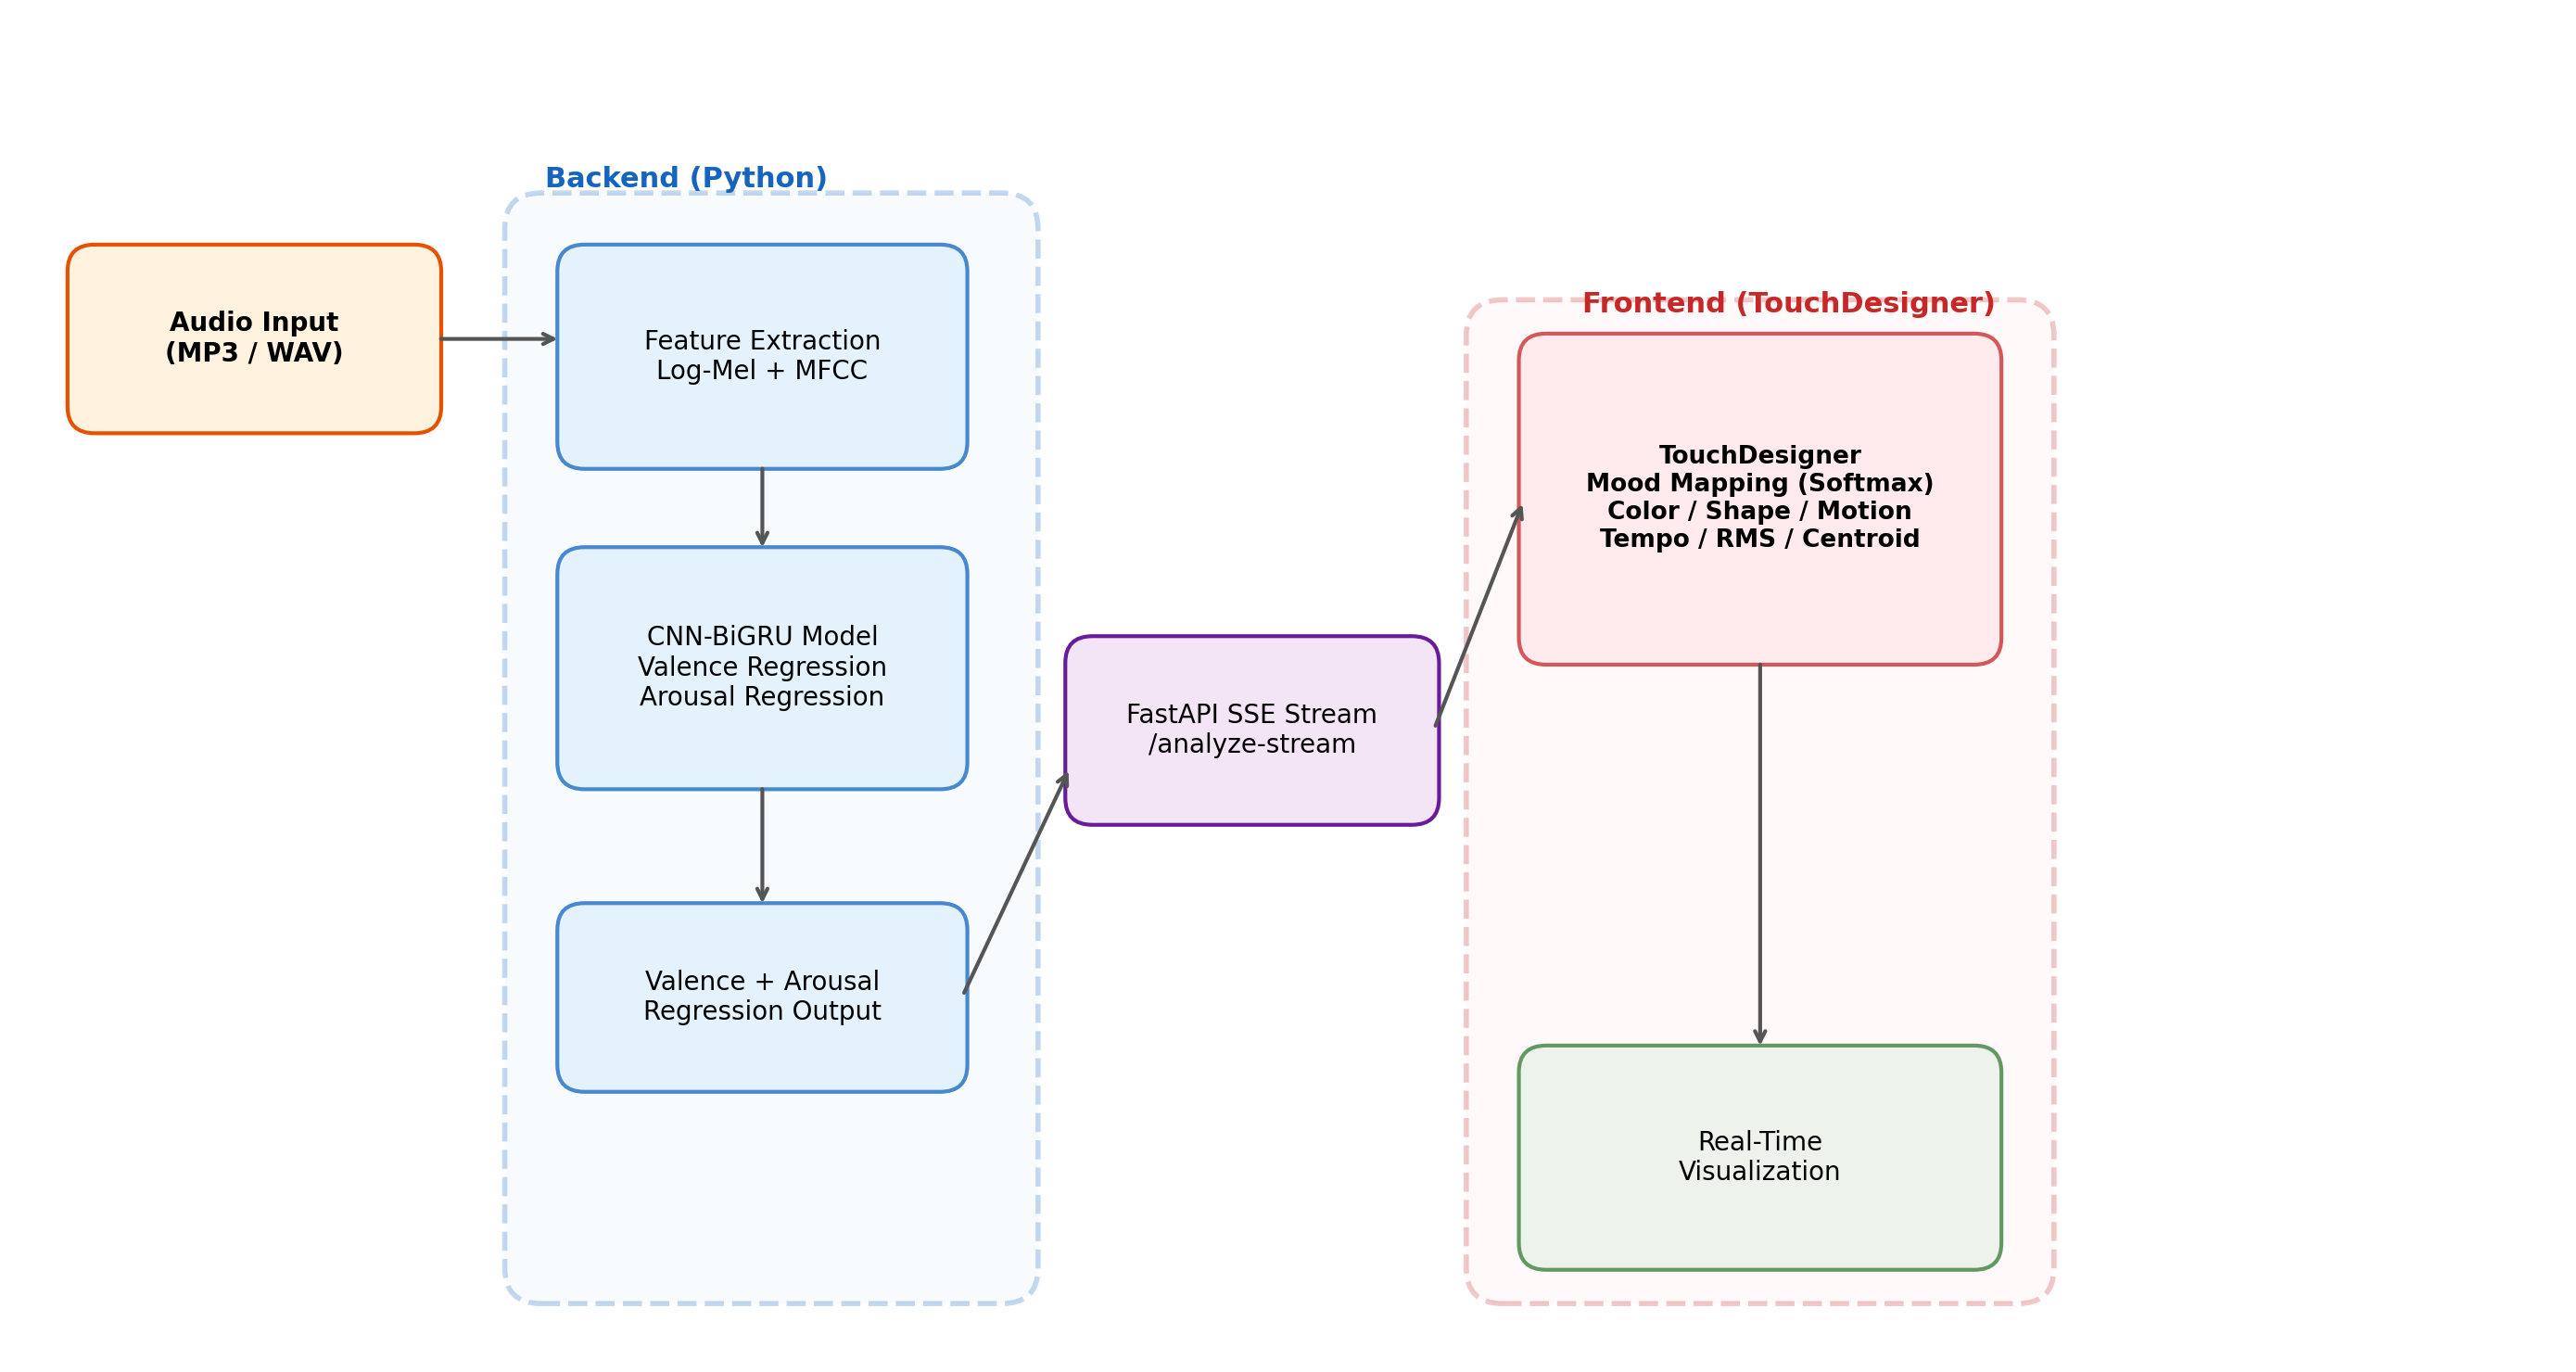
\includegraphics[width=\textwidth]{assets/architecture.png}
\caption{Overall system architecture of MoodWave, showing the data flow from raw audio input through the Python backend to the TouchDesigner visualization frontend.}
\label{fig:architecture}
\end{figure}

The pipeline operates as follows. The user provides an audio file (MP3 or WAV) to the backend through an HTTP POST request to the \texttt{/analyze-stream} endpoint. The backend loads the audio via Librosa and resamples it to 22,050~Hz if necessary. The feature extraction module computes log-Mel spectrograms and MFCCs across the entire audio stream, which are normalized using pre-computed training statistics (per-channel mean and standard deviation). The normalized segments are fed into the deep learning model, which outputs predicted valence and arousal values for the complete track. These continuous predictions are streamed to the frontend via the API. TouchDesigner then maps the valence-arousal pairs to a discrete mood distribution via a softmax over inverse distances to pre-defined mood prototypes in the valence-arousal plane. Additionally, TouchDesigner independently extracts lightweight acoustic features (tempo, RMS energy, spectral centroid) from the audio signal for creative modulation in the visualization. \\

All predictions are packaged into a JSON payload and streamed back to the client using \textbf{Server-Sent Events (SSE)}, a lightweight HTTP-based streaming protocol that allows the server to push the result to the client once inference is complete. The TouchDesigner frontend consumes this SSE stream, parses the JSON packets to obtain valence and arousal values, performs mood mapping to derive discrete mood labels, and routes these labels to texture-switching logic. Independently extracted RMS, tempo, and spectral centroid values drive geometry deformation and particle-system parameters. This decoupled architecture ensures that the computationally expensive deep learning inference remains on the backend (where GPU acceleration is available), while the frontend focuses exclusively on high-frame-rate real-time rendering. \\

\subsection{Key Technologies}

This subsection focuses exclusively on the backend technologies and algorithmic components under active development by the backend team.

\subsubsection{Deep Learning Framework: PyTorch}

The backend deep learning stack is built entirely on \textbf{PyTorch}, a dynamic computation graph framework that provides fine-grained control over model architecture, custom loss functions, and training loops. We chose PyTorch over alternatives such as TensorFlow because its eager execution mode simplifies debugging of complex multi-task architectures and facilitates rapid experimentation with custom attention mechanisms and data augmentation pipelines. The framework also offers seamless GPU acceleration via CUDA, which reduces inference latency from approximately 2--3 seconds per song on CPU to under 200 milliseconds on a mid-range NVIDIA GPU. \\

\subsubsection{Feature Extraction: Librosa}

\textbf{Librosa} is the backbone of our audio preprocessing pipeline. It handles audio loading, resampling, Mel spectrogram computation, MFCC extraction, tempo estimation, and RMS energy calculation through a unified, well-documented Python API. Librosa's default parameters are carefully tuned to music analysis tasks: we use an FFT window size of 2,048 samples, a hop length of 512 samples, and 64 Mel bands, yielding a spectrogram temporal resolution of approximately 23~ms per frame. This resolution strikes a balance between frequency localization (sufficient for timbre perception) and temporal smoothness (necessary for emotional continuity).

\subsubsection{MER Model Architecture 1: CNN-BiGRU with Attention}

The first architecture we developed is an end-to-end \textbf{CNN-BiGRU} model inspired by the end-to-end music emotion regression model proposed by Wu~\cite{wu2026}. The model ingests 2-channel log-Mel/MFCC segments and processes them through the following stages (see Figure~\ref{fig:model_architecture}).

\begin{figure}[htbp]
\centering
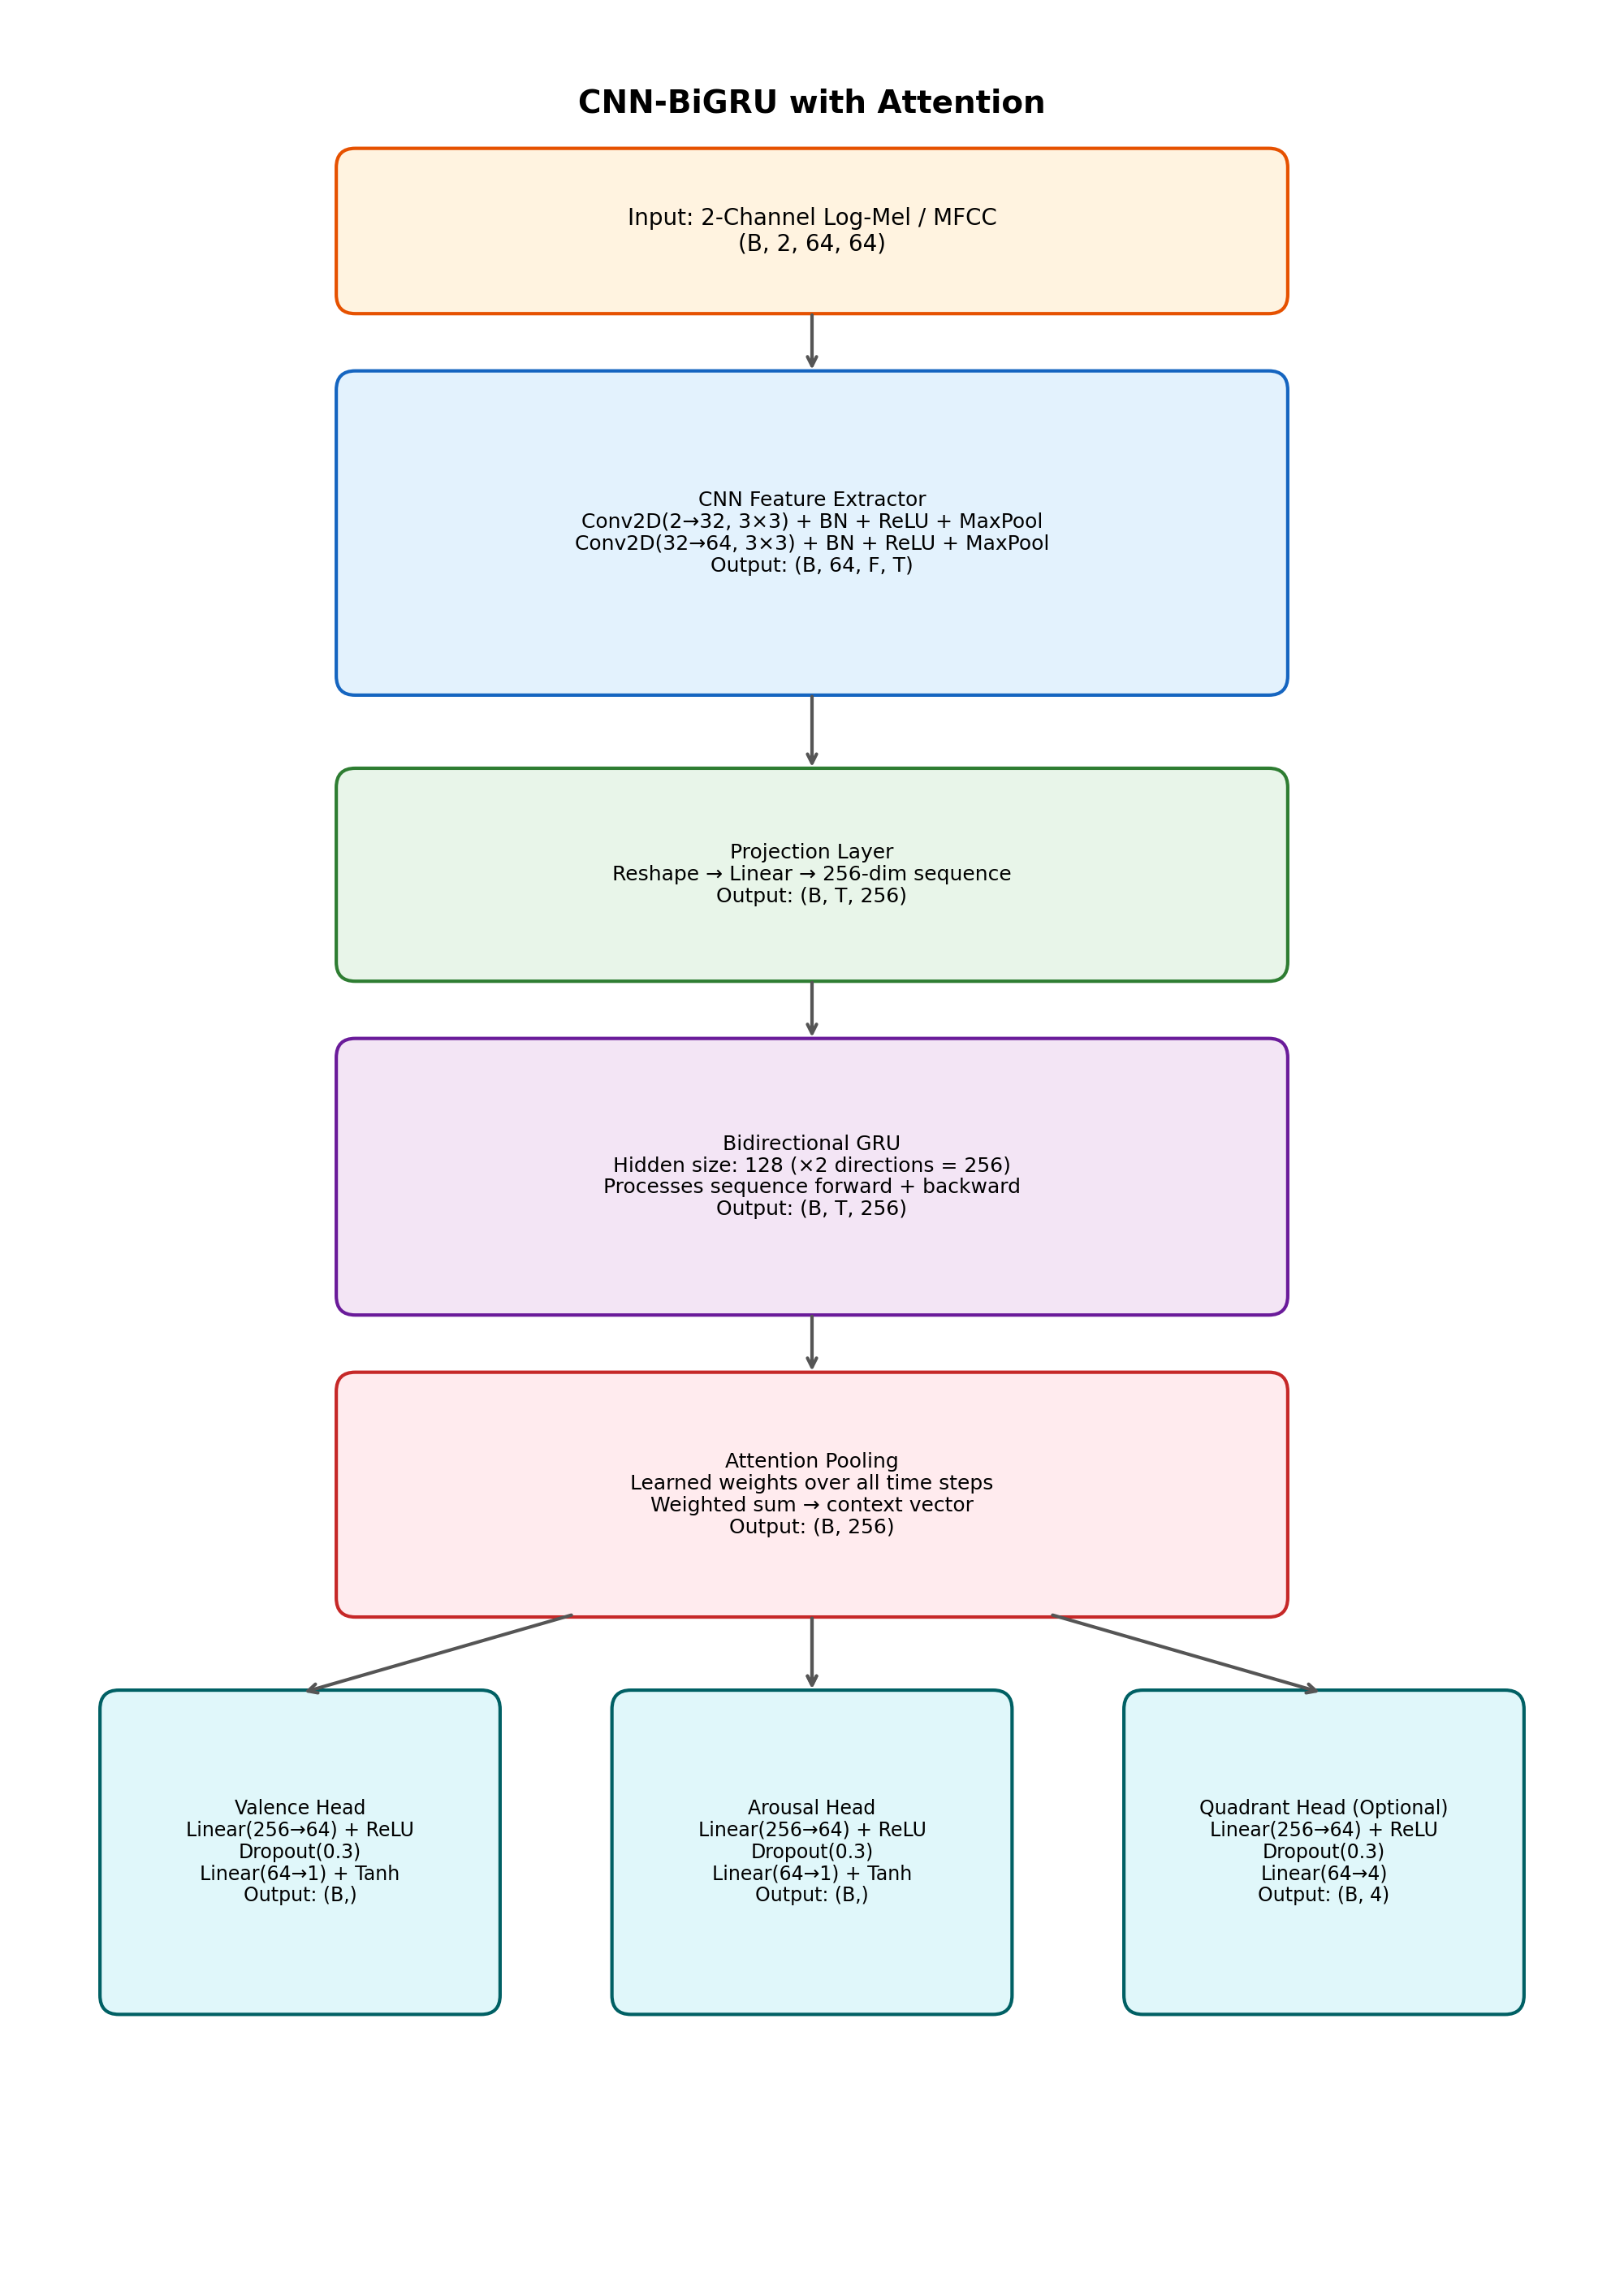
\includegraphics[width=0.75\textwidth]{assets/model_architecture.png}
\caption{Internal architecture of the CNN-BiGRU model with attention pooling and multi-task regression heads.}
\label{fig:model_architecture}
\end{figure}

\begin{enumerate}
    \item \textbf{Convolutional Feature Extractor:} Two 2-D convolutional layers with batch normalization and ReLU activation learn localized spectral patterns (e.g., harmonic structures, noise-like textures). For our \texttt{strict}-split experiments, we reduced filter counts from 32/64 to 16/32 to combat overfitting.
    
    \item \textbf{Projection Layer:} The CNN output is reshaped and projected into a lower-dimensional sequence representation suitable for recurrent processing.
    
    \item \textbf{Bidirectional GRU (BiGRU):} A bidirectional gated recurrent unit processes the projected sequence in both forward and backward directions. For the \texttt{strict} split, we reduced the hidden size from 128 to 64 as a regularization measure.
    
    \item \textbf{Attention Pooling:} Instead of using the final hidden state, we apply a learned attention mechanism that computes a weighted sum over all BiGRU time steps. The attention weights allow the model to focus selectively on emotionally salient frames.
    
    \item \textbf{Multi-Task Regression Heads:} Two separate fully-connected heads with Tanh output activation predict valence and arousal, respectively. An optional auxiliary \textbf{quadrant classification head} maps the pooled representation to one of four emotion quadrants, providing an additional supervised signal that regularizes the shared feature extractor.
\end{enumerate}

The model is trained with a \textbf{multi-task loss} combining Smooth L1 (Huber) losses for valence and arousal regression, optionally augmented with a cross-entropy term for quadrant classification. We employ the \textbf{AdamW} optimizer with a OneCycle learning rate scheduler, which linearly warms up the learning rate over the first 30\% of training steps before cosine annealing to a near-zero minimum. Gradient clipping at a maximum norm of 1.0 stabilizes training, while early stopping with a patience of 15 epochs prevents overfitting.

\subsubsection{MER Model Architecture 2: OpenL3-MLP Baseline}

To establish a strong baseline and diagnose the feature-learning bottleneck in our CNN-BiGRU, we implemented a second architecture based on \textbf{OpenL3} pre-trained audio embeddings. OpenL3 is a self-supervised contrastive model trained on millions of audio clips; its music-domain variant outputs 512-dimensional vectors that capture timbral, rhythmic, and high-level semantic information. We extract embeddings at a hop size of 0.5~seconds, aligning perfectly with DEAM's 2~Hz annotation rate. A lightweight \textbf{MLP} with two hidden layers (256 and 128 units, ReLU activation, dropout 0.2) maps each 512-dim embedding directly to valence and arousal. Notably, this model has only ~300K parameters and contains no recurrence or attention, yet it serves as a powerful benchmark because the heavy representational lifting is performed by the pre-trained encoder.

\subsubsection{Data Pipeline and Augmentation}

To improve generalization, the training pipeline incorporates several data augmentation strategies applied during segment extraction:
\begin{itemize}
    \item \textbf{Pitch shifting} ($\pm 2$ semitones): Simulates transposition and key changes.
    \item \textbf{Time stretching} ($0.9\times$, $1.1\times$): Simulates tempo variations while preserving pitch.
    \item \textbf{Noise injection} (Gaussian noise with $\sigma = 0.005 \cdot \max(|x|)$): Improves robustness to recording artifacts and compression noise.
\end{itemize}

At the batch level, we further apply random Gaussian noise, time-frame masking, and frequency-bin masking directly to the input tensors, following the SpecAugment paradigm adapted for music. For the \texttt{strict}-split CNN-BiGRU experiments, we made SpecAugment more aggressive (wider masks and random time warping) to combat overfitting on the smaller effective training set.

\subsubsection{API and Web Framework: FastAPI with Server-Sent Events}

The backend exposes its functionality through \textbf{FastAPI}, a modern asynchronous Python web framework built on Starlette and Pydantic. FastAPI automatically generates OpenAPI documentation, validates request schemas, and handles file uploads efficiently. The \texttt{/analyze-stream} endpoint accepts an audio file via multipart form upload and returns a \textbf{StreamingResponse} with MIME type \texttt{text/event-stream}. This SSE mechanism is chosen over WebSockets because our communication pattern is strictly unidirectional (server-to-client) and SSE integrates more naturally with TouchDesigner's HTTP-based DAT operators without requiring persistent socket management.

\subsubsection{Dataset: DEAM and Evaluation Protocols}

We train and evaluate our models on the \textbf{DEAM} dataset. The dataset is split into training (70\%), validation (15\%), and test (15\%) sets. We report performance at two granularities. At the \textbf{frame/segment level}, we evaluate every prediction against the corresponding annotation using Mean Absolute Error (MAE), coefficient of determination ($R^2$), and quadrant classification accuracy. At the \textbf{track level}, we average all predictions within a song and compare them to the track's mean ground-truth valence and arousal. For the OpenL3-MLP model, we additionally report Root Mean Square Error (RMSE) and Pearson Correlation Coefficient (PCC), following the evaluation protocol of the reference paper~\cite{lyu2026}.

% ============================================================
\section{Midterm Progress and Milestone Achievements}
% ============================================================

At the midterm deadline, we have completed the full backend training pipeline, implemented two distinct model architectures, conducted a rigorous evaluation comparing track-level and segment-level splits, and integrated a real-time inference API. The following subsections summarize our experimental results and quantitative findings.

\subsection{Experimental Setup}

All experiments were conducted on a server equipped with an NVIDIA GPU and CUDA 12.1. The CNN-BiGRU was trained with the AdamW optimizer, OneCycleLR scheduler (max LR $1\times10^{-4}$, warm-up 30\%), and gradient clipping (max norm 1.0). The OpenL3-MLP used AdamW at $5\times10^{-4}$ with batch size 156. Both models employ early stopping with patience 15. For the CNN-BiGRU \texttt{strict}-split run, we applied heavier regularization (dropout 0.7, weight decay $10^{-2}$, reduced filters 16/32, hidden size 64) and increased segment length from 1.5~s to 10~s to provide more musical context.

\subsection{Quantitative Results}

Table~\ref{tab:results} presents the comprehensive comparison across both architectures and both splitting strategies.

\begin{table}[htbp]
\centering
\caption{Test-set performance comparison. CNN-BiGRU \texttt{paper} uses 1.5~s segments; CNN-BiGRU \texttt{strict} uses 10~s segments with stronger regularization. OpenL3-MLP operates on 0.5~s frame-level embeddings.}
\label{tab:results}
\small
\begin{tabular}{@{}l l c c c c c c@{}}
\toprule
\textbf{Model} & \textbf{Split} & \textbf{V-MAE$\downarrow$} & \textbf{V-$R^2$$\uparrow$} & \textbf{A-MAE$\downarrow$} & \textbf{A-$R^2$$\uparrow$} & \textbf{Q-Acc$\uparrow$} & \textbf{Trk-Q-Acc$\uparrow$} \\
\midrule
CNN-BiGRU & \texttt{paper} & 0.054 & \textbf{0.914} & 0.062 & \textbf{0.891} & 0.860 & \textbf{0.957} \\
CNN-BiGRU & \texttt{strict} & 0.151 & 0.399 & 0.142 & 0.559 & 0.616 & 0.701 \\
\midrule
OpenL3-MLP & \texttt{paper} & 0.088 & 0.788 & 0.090 & 0.825 & 0.783 & 0.863 \\
OpenL3-MLP & \texttt{strict} & 0.161 & 0.322 & 0.139 & 0.606 & 0.592 & 0.686 \\
\bottomrule
\end{tabular}
\end{table}

\textbf{Key observations from Table~\ref{tab:results}:}

\begin{enumerate}
    \item \textbf{Data leakage is severe.} The \texttt{paper} split, which allows segments from the same song to leak into the test set, produces unrealistically high metrics for both models. The CNN-BiGRU achieves track-level $R^2$ of 0.987 and 0.991 for valence and arousal---not because it understands emotion, but because it memorizes song-specific acoustic fingerprints.
    
    \item \textbf{Strict split reveals true generalization.} Under honest track-level separation, CNN-BiGRU performance drops dramatically (track $R^2$ falls from 0.987 to 0.552 for valence). This confirms that learning features from scratch on only 1,800 songs is extremely difficult.
    
    \item \textbf{OpenL3 generalizes better.} On the honest \texttt{strict} split, OpenL3-MLP achieves track arousal $R^2$ of 0.754 versus CNN-BiGRU's 0.726, despite having only 300K parameters and no recurrence. The pre-trained embeddings encode robust musical semantics that transfer well to unseen songs.
    
    \item \textbf{Arousal is easier than valence.} Across all configurations, arousal $R^2$ is consistently higher than valence $R^2$. This aligns with prior work: arousal correlates strongly with acoustic attributes such as tempo, RMS energy, and spectral centroid, whereas valence depends on more subtle harmonic and lyrical cues.
\end{enumerate}

\subsection{Training Curves and Visualizations}

Figure~\ref{fig:cnn_loss} shows the training and validation loss trajectories for the CNN-BiGRU under both splitting modes. Under the \texttt{paper} split, validation loss closely tracks training loss, suggesting good fit---but this is illusory because the validation set contains familiar songs. Under the \texttt{strict} split, a clear generalization gap emerges after epoch 20, indicating that the model begins to overfit to training-song patterns that do not transfer.

\begin{figure}[htbp]
\centering
\begin{subfigure}[b]{0.48\textwidth}
    \centering
    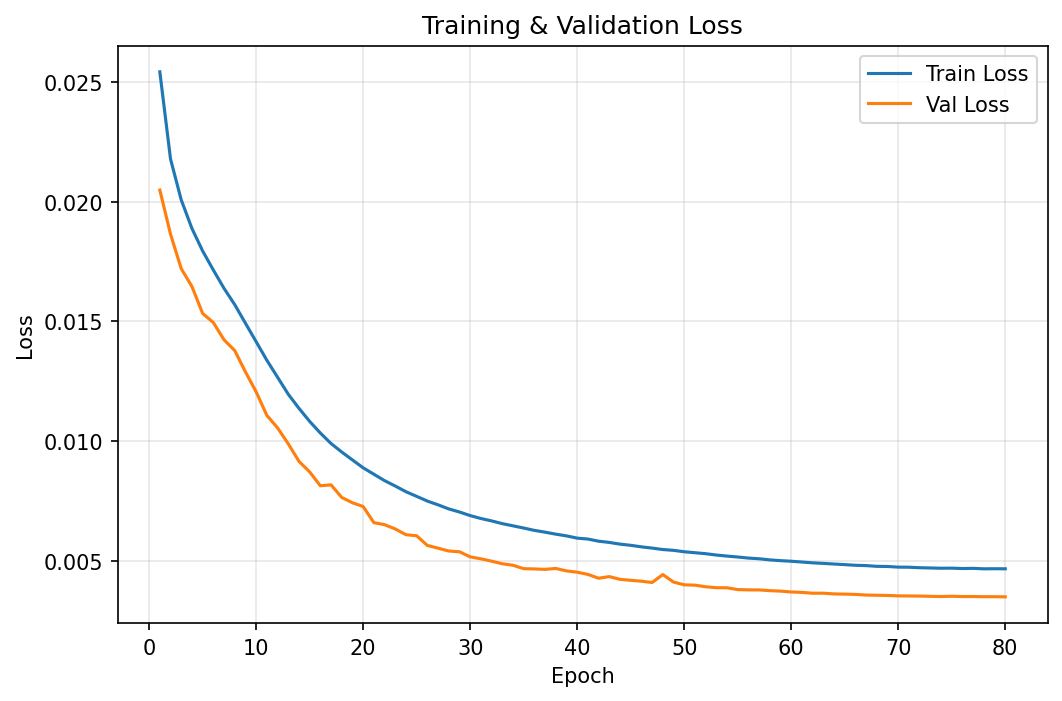
\includegraphics[width=\textwidth]{assets/cnn_paper_loss.png}
    \caption{CNN-BiGRU \texttt{paper} split}
\end{subfigure}
\hfill
\begin{subfigure}[b]{0.48\textwidth}
    \centering
    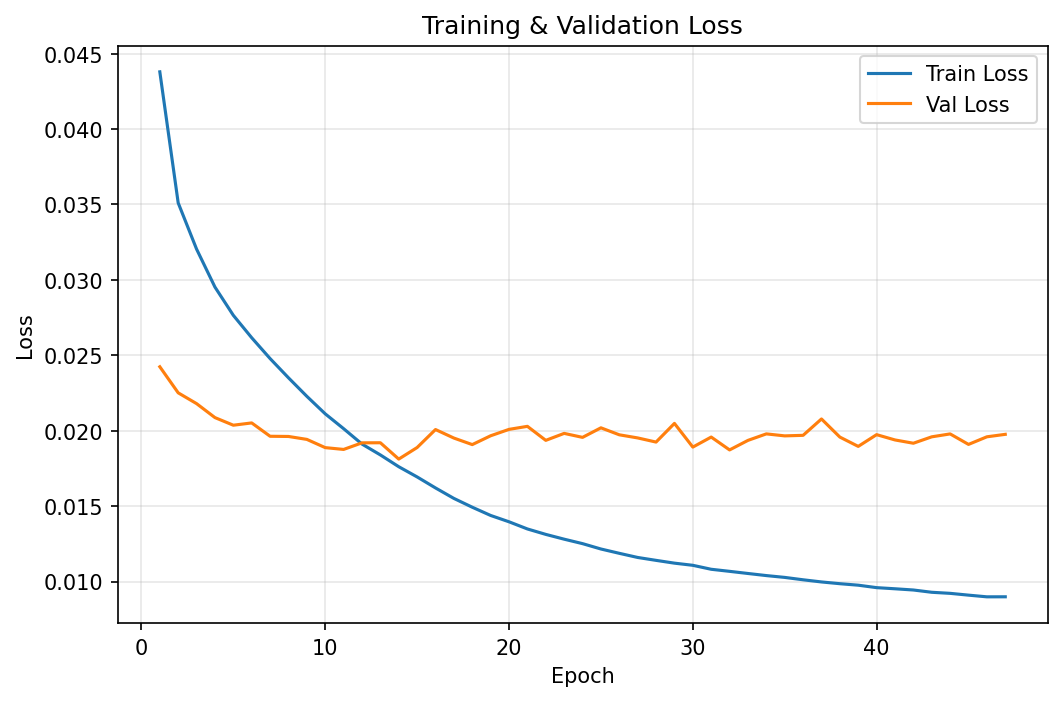
\includegraphics[width=\textwidth]{assets/cnn_strict_loss.png}
    \caption{CNN-BiGRU \texttt{strict} split}
\end{subfigure}
\caption{Training vs. validation loss curves for CNN-BiGRU. The \texttt{strict} split reveals a significant generalization gap after epoch 20.}
\label{fig:cnn_loss}
\end{figure}

Figure~\ref{fig:cnn_r2} displays the validation $R^2$ progression. The \texttt{paper} split saturates near-perfect $R^2$ within 10 epochs, while the \texttt{strict} split plateaus around 0.4--0.5 for valence and 0.5--0.6 for arousal.

\begin{figure}[htbp]
\centering
\begin{subfigure}[b]{0.48\textwidth}
    \centering
    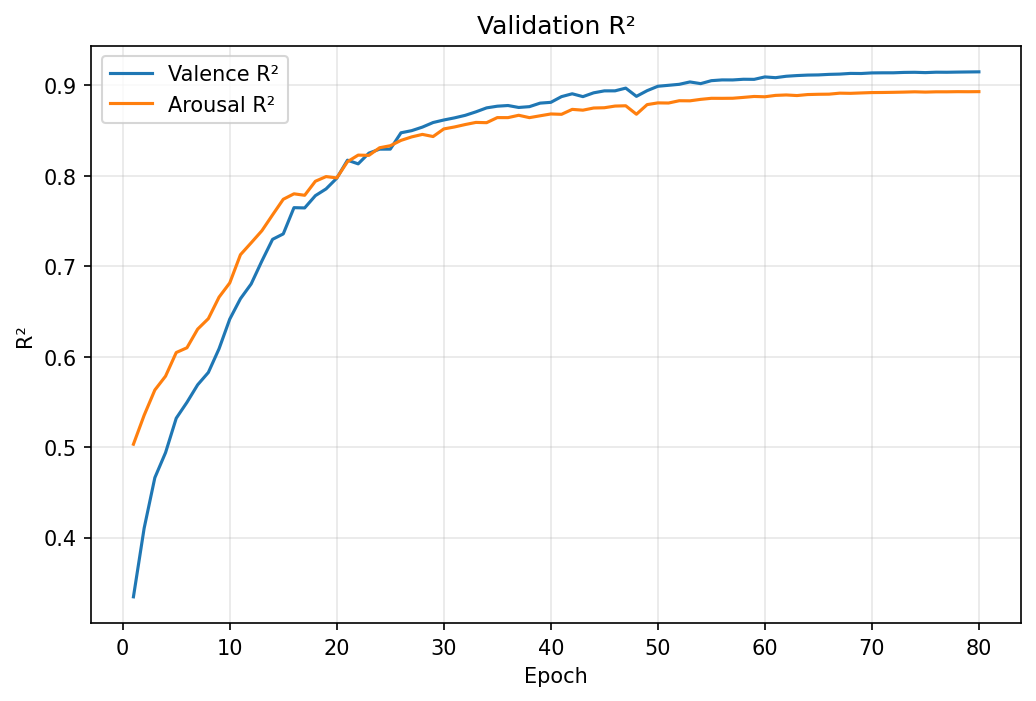
\includegraphics[width=\textwidth]{assets/cnn_paper_r2.png}
    \caption{CNN-BiGRU \texttt{paper} split}
\end{subfigure}
\hfill
\begin{subfigure}[b]{0.48\textwidth}
    \centering
    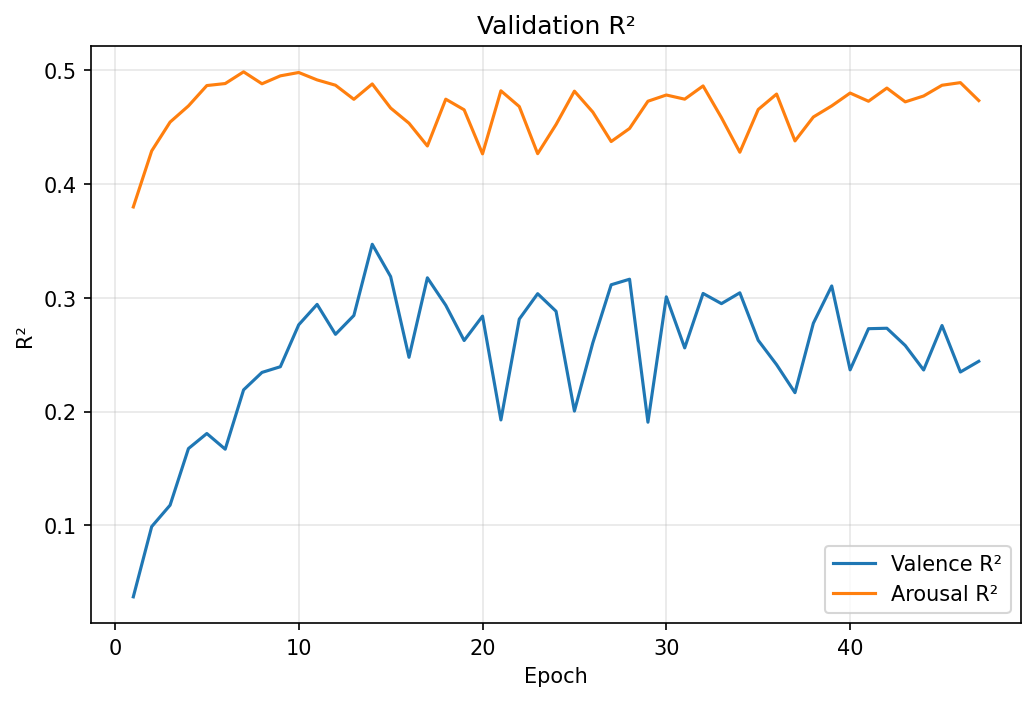
\includegraphics[width=\textwidth]{assets/cnn_strict_r2.png}
    \caption{CNN-BiGRU \texttt{strict} split}
\end{subfigure}
\caption{Validation $R^2$ curves for CNN-BiGRU. The \texttt{paper} split saturates unrealistically fast due to data leakage.}
\label{fig:cnn_r2}
\end{figure}

For the OpenL3-MLP baseline, Figure~\ref{fig:openl3_pcc} presents the Pearson correlation coefficients on the validation set. Under the \texttt{paper} split, the model achieves PCC $\approx$ 0.89 for valence and 0.91 for arousal, closely matching the reference paper's reported values (0.878 and 0.909). Under the \texttt{strict} split, PCC drops to roughly 0.58 and 0.72, confirming that even strong pre-trained features cannot fully compensate for the train-test domain shift when songs are completely unseen.

\begin{figure}[htbp]
\centering
\begin{subfigure}[b]{0.48\textwidth}
    \centering
    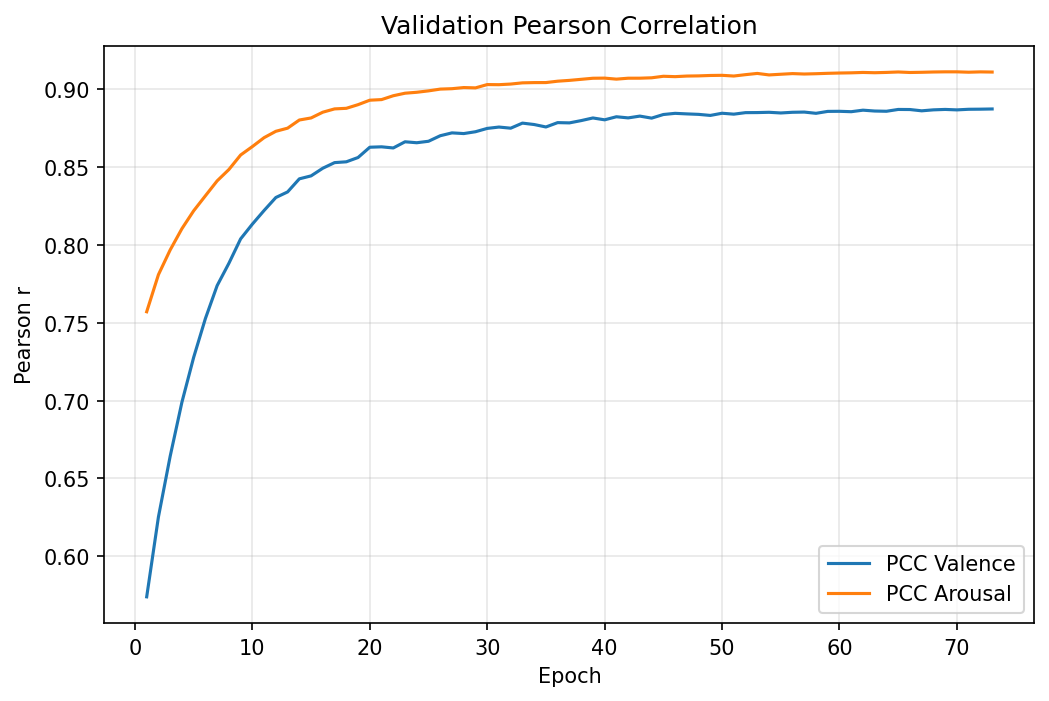
\includegraphics[width=\textwidth]{assets/openl3_paper_pcc.png}
    \caption{OpenL3-MLP \texttt{paper} split}
\end{subfigure}
\hfill
\begin{subfigure}[b]{0.48\textwidth}
    \centering
    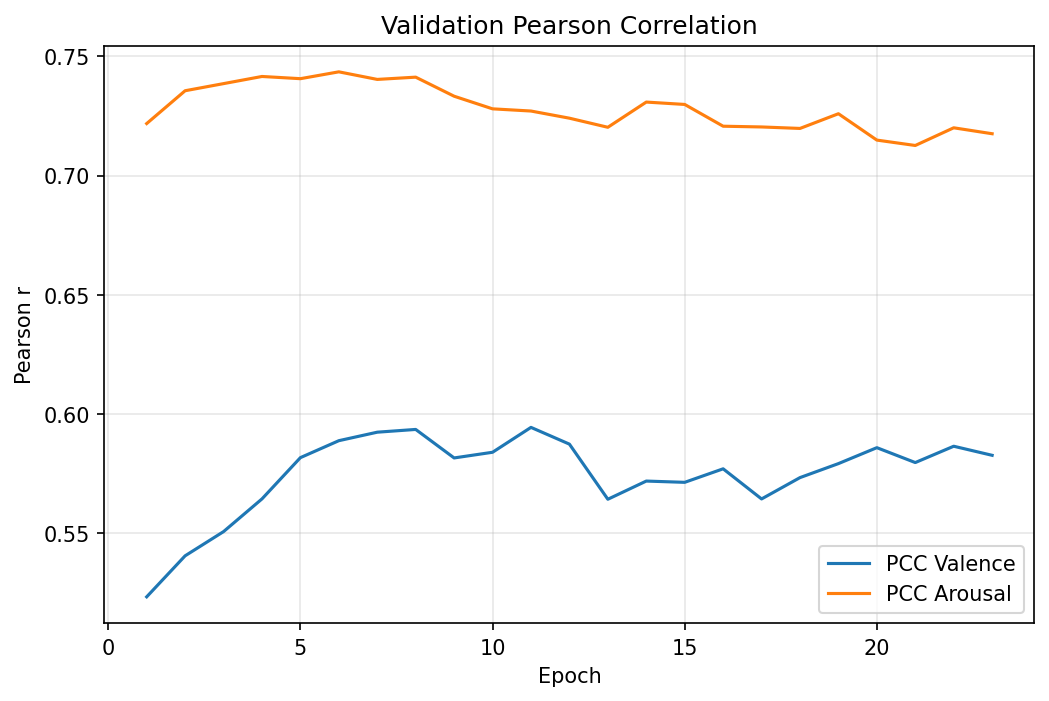
\includegraphics[width=\textwidth]{assets/openl3_strict_pcc.png}
    \caption{OpenL3-MLP \texttt{strict} split}
\end{subfigure}
\caption{Validation Pearson correlation curves for OpenL3-MLP.}
\label{fig:openl3_pcc}
\end{figure}

Finally, Figure~\ref{fig:track_r2} compares track-level $R^2$ for both models under the \texttt{strict} split. Track-level aggregation (averaging predictions per song before scoring) consistently improves $R^2$ by 0.1--0.2 points because frame-level noise cancels out during averaging.

\begin{figure}[htbp]
\centering
\begin{subfigure}[b]{0.48\textwidth}
    \centering
    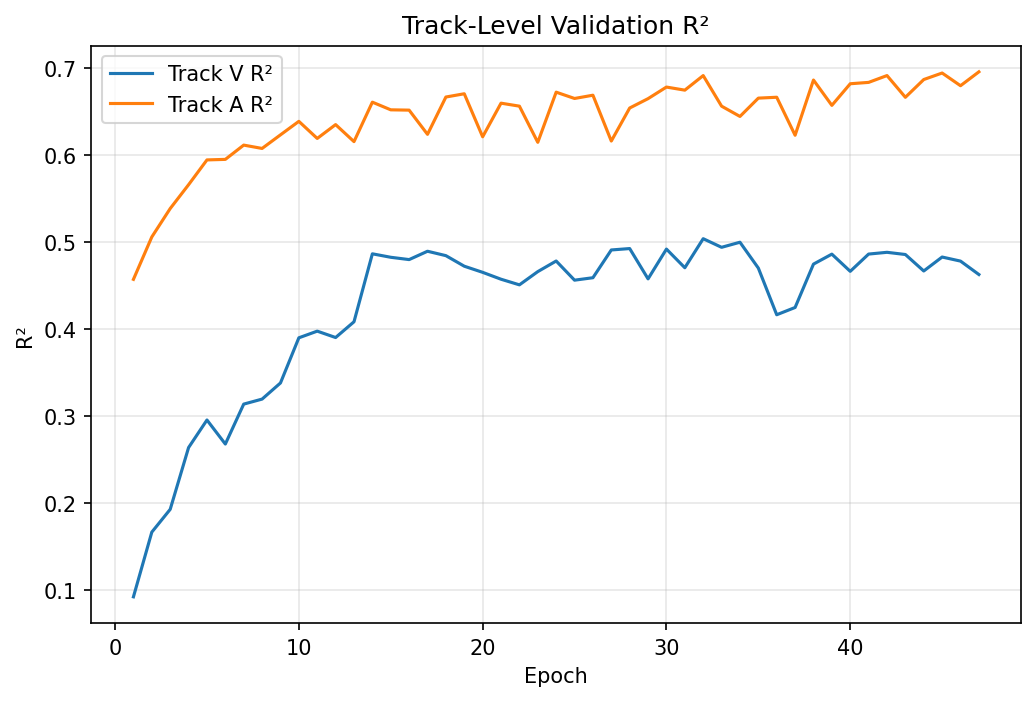
\includegraphics[width=\textwidth]{assets/cnn_strict_track_r2.png}
    \caption{CNN-BiGRU \texttt{strict}}
\end{subfigure}
\hfill
\begin{subfigure}[b]{0.48\textwidth}
    \centering
    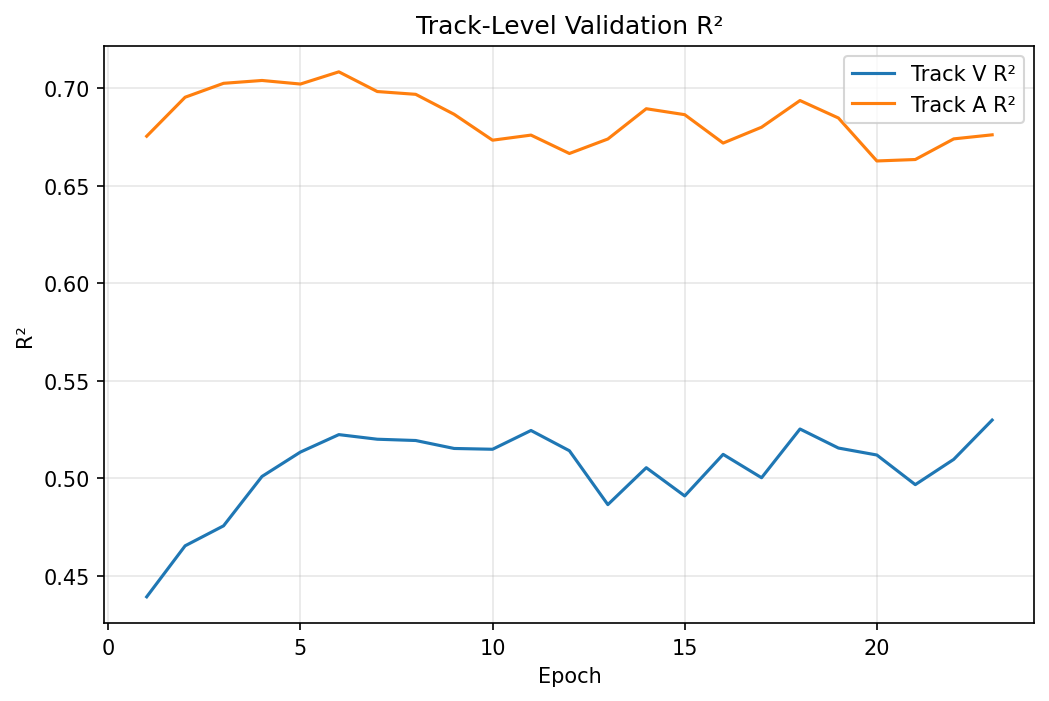
\includegraphics[width=\textwidth]{assets/openl3_strict_track_r2.png}
    \caption{OpenL3-MLP \texttt{strict}}
\end{subfigure}
\caption{Track-level validation $R^2$ curves under honest track-level splitting.}
\label{fig:track_r2}
\end{figure}

\subsection{Milestone Checklist}

\begin{itemize}
    \item[$\checkmark$] DEAM dataset ingestion and dynamic annotation alignment
    \item[$\checkmark$] CNN-BiGRU architecture with attention pooling and multi-task heads
    \item[$\checkmark$] OpenL3-MLP baseline for comparative analysis
    \item[$\checkmark$] Training pipeline with OneCycleLR, gradient clipping, and early stopping
    \item[$\checkmark$] Per-epoch metrics logging and automatic plot generation
    \item[$\checkmark$] Track-level vs. segment-level evaluation protocols
    \item[$\checkmark$] FastAPI inference endpoint with SSE streaming
    \item[$\checkmark$] Lion Swarm Optimization (LSO) module for automated hyperparameter search
    \item[$\square$] TouchDesigner frontend integration (in progress)
    \item[$\square$] Real-time demo video (planned for final deliverable)
    \item[$\square$] PMEmo2019 dataset integration for cross-dataset generalization (future work)
\end{itemize}

% ============================================================
\section{Challenges and Solutions}
% ============================================================

\subsection{Challenge 1: Severe Data Leakage in Standard Splits}

\textbf{Problem:} Our initial experiments followed the ``paper'' split described in Wu~\cite{wu2026}, which stratifies individual mel-segments by quadrant. We observed suspiciously high test metrics ($R^2 > 0.9$) and suspected data leakage. Upon investigation, we discovered that because DEAM provides multiple segments per song, the stratified shuffle places segments from the same song into both training and test sets. Since adjacent mel-spectrogram segments are highly correlated, the model effectively memorizes song-specific acoustic patterns rather than learning generalizable emotion cues. \\

\textbf{Solution:} We implemented a \texttt{strict} track-level split that assigns all segments (or frames) from a single song to exactly one fold. Comparing \texttt{paper} vs. \texttt{strict} splits revealed a catastrophic drop in performance (e.g., CNN-BiGRU valence $R^2$ fell from 0.914 to 0.399), confirming that prior literature's reported numbers are heavily inflated by leakage. All subsequent honest evaluations use the \texttt{strict} split exclusively.

\subsection{Challenge 2: Memory Explosion with Long Segments}

\textbf{Problem:} To provide more musical context, we increased segment length from 1.5~s to 10~s (430 spectrogram frames). However, the extraction code was still generating one segment per annotation timestamp (every 0.5~s), leading to 60 massive, nearly identical 10-second segments per song. During cache construction, memory usage ballooned to over 170~GB and triggered an out-of-memory kill. \\

\textbf{Solution:} We introduced a configurable minimum hop ($MEL\_SEGMENT\_HOP\_S = 3.0$~s) between extracted segment centers, reducing the count from ~60 to ~10 segments per song. We also added incremental chunk saving (flushing partial \texttt{.npz} caches every 200 songs), which caps peak memory regardless of dataset size. Post-fix memory usage stayed below 25~GB.

\subsection{Challenge 3: CNN-BiGRU Overfitting on Small Data}

\textbf{Problem:} Under the honest \texttt{strict} split, our CNN-BiGRU severely overfitted. With only ~1,260 training songs and a ~2M-parameter model, the network learned song-specific timbral artifacts rather than general emotion rules. Validation metrics plateaued early and then degraded. \\

\textbf{Solution:} We applied a suite of regularization measures: (1) reduced model capacity (filters 16/32, hidden size 64, dropout 0.7); (2) increased weight decay to $10^{-2}$; (3) aggressive SpecAugment with wider time/frequency masking and random time warping; (4) longer 10~s segments to force the model to attend to musical phrase structure. These changes improved strict-split track-level quadrant accuracy from an estimated baseline of ~55\% to 70.1\%.

\subsection{Challenge 4: Feature Representation Bottleneck}

\textbf{Problem:} Even with heavy regularization, the CNN-BiGRU struggled to generalize. The gap between our best honest CNN-BiGRU results (track $R^2$ ~0.55 for valence) and the OpenL3-MLP baseline (track $R^2$ ~0.52 for valence, but much better for arousal at 0.75) suggests that the primary bottleneck is \textit{feature quality}, not architecture. Learning meaningful musical representations from scratch on 1,800 songs is fundamentally harder than leveraging embeddings pre-trained on millions of audio clips. \\

\textbf{Solution:} We identified that the primary bottleneck is \textit{feature quality}, not architectural capacity. Rather than abandoning the CNN-BiGRU, we will implement \textbf{stronger pre-trained encoder baselines} using modern audio foundation models---specifically CLAP (Contrastive Language-Audio Pretraining) \cite{clap2023} and MuQ (Mel Residual Vector Quantization with Conformer) \cite{muq2025}---and use them as reference ``teacher'' models. Insights from these stronger baselines (e.g., via knowledge distillation, feature fusion, or comparative error analysis) will directly guide further improvements to our custom CNN-BiGRU architecture. This ``strong baseline $\rightarrow$ custom model improvement'' pipeline ensures that our final system retains the interpretability and efficiency of an end-to-end design while closing the generalization gap with state-of-the-art pre-trained representations.

% ============================================================
\section{Future Work}
% ============================================================

Based on the midterm findings, we have identified four priority directions for the remainder of the semester: (1) implementing stronger pre-trained encoder baselines (CLAP, MuQ) and leveraging them to improve our custom CNN-BiGRU, (2) completing the TouchDesigner frontend integration, (3) expanding evaluation to cross-dataset generalization, and (4) delivering the real-time demonstration video. Table~\ref{tab:future} summarizes the planned milestones, timeline, and team assignments.

\begin{table}[htbp]
\centering
\caption{Future work plan from midterm to final deliverable (April--June 2026).}
\label{tab:future}
\small
\begin{tabular}{@{}p{2.2cm}p{4.8cm}p{3.5cm}p{2.5cm}@{}}
\toprule
\textbf{Week} & \textbf{Task / Milestone} & \textbf{Deliverable} & \textbf{Owner} \\
\midrule
\textbf{W1--W2} & \textit{Stronger baselines.} Implement CLAP and MuQ encoder baselines; evaluate their strict-split performance against OpenL3-MLP. Use comparative analysis and knowledge distillation to improve the custom CNN-BiGRU. Retrain with LSO and export ONNX. & Improved CNN-BiGRU checkpoint; inference latency $<$ 200 ms & Member A \\
\midrule
\textbf{W3--W4} & \textit{Frontend integration.} Implement TouchDesigner DAT operator to consume SSE stream from FastAPI. Map valence/arousal to color palettes, particle dynamics, and geometry deformation. & Working TD patch with real-time reactivity & Member B \\
\midrule
\textbf{W5--W6} & \textit{Cross-dataset validation.} Integrate PMEmo2019 as a secondary test set. Evaluate zero-shot transfer of the OpenL3-MLP model and report generalization gap. & PMEmo2019 evaluation report & Member C \\
\midrule
\textbf{W7--W8} & \textit{Demo video \& documentation.} Record a 3-minute demonstration showing live audio input, backend prediction, and TD visualization. Prepare final report and GitHub documentation. & Demo video + final report & All members \\
\bottomrule
\end{tabular}
\end{table}

\subsection{Stronger Baseline Encoders and CNN-BiGRU Improvement}

The midterm experiments show that pre-trained features (OpenL3) generalize better than features learned from scratch on 1,800 songs. However, OpenL3 is not the strongest available audio encoder. We will therefore implement two modern foundation-model baselines: \textbf{CLAP} (Contrastive Language-Audio Pretraining, 512--1024~dim) \cite{clap2023} and \textbf{MuQ} (Conformer-based masked token prediction, 4096~dim frame features) \cite{muq2025}. These models were pre-trained on orders of magnitude more data (630K+ audio-text pairs for CLAP; 130K+ hours of music for MuQ) and capture richer semantic, timbral, and structural cues than OpenL3.

Rather than replacing the CNN-BiGRU outright, we will use these stronger baselines as \textit{reference teachers} to improve our custom model. Specifically, we will explore three transfer strategies:
\begin{enumerate}
    \item \textbf{Knowledge distillation:} Train the CNN-BiGRU to match the soft regression targets produced by the frozen CLAP or MuQ encoder, providing an additional supervisory signal beyond the sparse DEAM annotations.
    \item \textbf{Feature fusion:} Concatenate or cross-attend between the CNN-BiGRU's convolutional features and a lightweight projection of the pre-trained embeddings, allowing the model to combine local spectral detail with high-level semantic context.
    \item \textbf{Comparative error analysis:} Identify song classes or emotional regions where the CNN-BiGRU fails but the foundation models succeed, then target those regions with hard-example mining or specialized augmentation.
\end{enumerate}
The improved CNN-BiGRU remains our target production architecture because it is fully differentiable end-to-end and does not require loading a massive pre-trained encoder at inference time. We will run Lion Swarm Optimization (LSO) over the improved architecture's hyperparameters using the \texttt{strict} split as the validation criterion, and export the final checkpoint to ONNX for sub-200~ms inference.

\subsection{TouchDesigner Frontend Integration}

The frontend team will develop a custom TouchDesigner DAT operator that establishes an HTTP connection to the \texttt{/analyze-stream} endpoint and parses Server-Sent Events (SSE). Valence and arousal values will drive three visual subsystems: (1) \textbf{color mapping} (warm/cool palette interpolation), (2) \textbf{particle dynamics} (speed and density modulated by arousal), and (3) \textbf{geometry deformation} (shape complexity linked to valence magnitude). Independently extracted tempo, RMS energy, and spectral centroid will provide secondary modulation parameters.

\subsection{Cross-Dataset Generalization with PMEmo2019}

To assess robustness beyond DEAM, we will integrate the \textbf{PMEmo2019} dataset, which contains 794 popular music excerpts annotated with both static and dynamic valence-arousal labels. Because PMEmo2019 uses a different annotation protocol and genre distribution, it serves as a challenging out-of-domain test. We will evaluate \textbf{all} our models---the new CLAP/MuQ baselines, the improved CNN-BiGRU, and the OpenL3-MLP reference---in a \textbf{zero-shot transfer} setting (no fine-tuning on PMEmo2019) to quantify the true generalization capability of each representation. If a significant domain gap exists, we will experiment with lightweight domain-adaptation techniques such as batch normalization tuning or adapter layers.

\subsection{Limitations and Risk Mitigation}

Two primary risks remain. First, TouchDesigner's HTTP DAT operators have limited async support; if SSE streaming proves unstable, we will fall back to polling the REST endpoint at 2~Hz intervals. Second, PMEmo2019 audio files are not freely redistributable; if access is delayed, we will substitute the \textbf{EmoMusic} dataset as an alternative cross-validation source. Both fallback plans are fully compatible with the existing pipeline and require no architectural changes.

% ============================================================
\section{Personal Reflection}
% ============================================================

\textbf{Vincent Ma}

Taking this course has been a genuinely valuable experience for understanding how modern encoder-based models work in media processing. The curriculum provides foundational knowledge that I believe is essential for anyone planning to pursue more advanced coursework---such as Deep Learning---or undertake an Innovation Project in the future. What I particularly appreciate is the course's emphasis on \textit{project-driven learning}: by allowing each student to research and develop a project in their own area of interest, the course naturally teaches how contemporary media-processing pipelines are designed, implemented, and evaluated in practice. Researching the MoodWave project forced me to confront real-world problems---memory constraints, data leakage, and feature-representation bottlenecks---that no textbook exercise could fully replicate.

For the second half of the semester, my suggestion is simply to maintain this project-centric approach. Continuing to develop and refine our own research gives us the opportunity to cultivate foundational research skills---experimental design, rigorous evaluation, and iterative debugging---that will be indispensable during graduate studies or a Ph.D. As the saying goes, one truly learns by doing.

From a technical standpoint, this project has deepened my understanding of audio and music encoders in several concrete ways. I designed and implemented the CNN-BiGRU encoder from scratch, giving me first-hand insight into how convolutional front-ends extract local spectral patterns and how bidirectional recurrent layers model temporal dynamics. I also explored optimization beyond standard gradient descent by integrating Lion Swarm Optimization (LSO) into our hyperparameter search pipeline. Perhaps the most important lesson, however, was discovering the danger of \textbf{data leakage}: the stark performance gap between our ``paper'' split and our honest ``strict'' split taught me that inflated metrics are essentially a lie about generalization, and that strict train-test separation is absolutely necessary in any credible machine-learning study.

% ============================================================
\section*{References}
% ============================================================

\begin{thebibliography}{9}

\bibitem{wu2026}
M.~Wu, ``Construction of music emotion recognition and classification model supported by neural networks,'' \emph{Journal on Audio, Speech, and Music Processing}, 2026. \url{https://doi.org/10.1186/s13636-026-00453-6}

\bibitem{lyu2026}
J.~Lyu, ``Music Emotion Regression Based on OpenL3 Embeddings,'' \emph{Proceedings of ICLLCD 2026 Symposium}, 2026. \url{https://doi.org/10.54254/2753-7064/2026.HT31555}

\bibitem{russell1980}
J.~A. Russell, ``A circumplex model of affect,'' \emph{Journal of Personality and Social Psychology}, vol.~39, no.~6, pp.~1161--1178, 1980.

\bibitem{deam2018}
M.~Soleymani, A.~Aljanaki, and Y.-H.~Yang, ``DEAM: MediaEval database for emotional analysis in music,'' University of Geneva and Academia Sinica, Switzerland, 2018.

\bibitem{openl3}
A.~Cramer, H.-H.~Wu, J.~Salamon, and J.~P.~Bello, ``Look, listen, and learn more: Design choices for deep audio embeddings,'' in \emph{Proc. IEEE ICASSP}, pp.~3852--3856, 2019.

\bibitem{mert2023}
Y.~Li et al., ``MERT: Acoustic Music Understanding Model with Large-Scale Self-supervised Training,'' \emph{arXiv preprint arXiv:2306.00107}, 2023.

\bibitem{pmemo2019}
E.~Y.~Koh et al., ``MERP: A Music Dataset with Emotion Ratings and Raters' Profile Information,'' \emph{Sensors}, vol.~23, no.~1, p.~382, 2022.

\bibitem{clap2023}
B.~Elizalde et al., ``CLAP: Learning audio concepts from natural language supervision,'' in \emph{Proc. IEEE ICASSP}, pp.~1--5, 2023.

\bibitem{muq2025}
Q.~Zhu et al., ``Self-Supervised Music Representation Learning with Mel Residual Vector Quantization,'' \emph{arXiv preprint arXiv:2501.01108}, 2025.

\end{thebibliography}

\end{document}
